% !Mode:: "TeX:UTF-8"
\section{实标量场: 零自旋有质量无荷, $\pi^0$ 介子}
\subsection{标量场的方程: Klein-Gordon 方程; 解中负能项的出现, 产生湮灭算符诠释}
狭义相对论中, 我们已知能动关系为~$p^2-m^2=0$; 量子力学中, 我们已知从经典到量子的一般代换原则为~$p^\mu=i\partial^\mu,~p_\mu=i\partial_\mu$; 据此, 我们可得方程
\begin{align}
(\partial^2+m^2)\phi(x)=0;
\end{align}
称为~Klein-Gordon 方程. 此方程, 是无论是洛伦兹标量, 矢量还是旋量, 都必然满足的; 具体地, 矢量与标量还满足更强要求的式子; 只满足上式而无更强关系的--也就是本章将研究的场, 则只是自旋为~0 的标量场. 第二点, 场方程中含有质量项, 这表示对应粒子有质量.

下面研究方程的解. 由方程的形式可看出, 它有可由两部分平面波构成, 分别是~$\propto e^{-ip^\mu x_\mu}$ 的--称为正能解, 与~$\propto e^{ip^\mu x_\mu}$ 的--称为负能解. 由前二平面波叠加成的~K-G 方程的一般解为
\begin{align}\label{so of kg}
\phi(x)&=\int\frac{d^3\bm{p}}{(2\pi)^3\sqrt{2E_{\bm{p}}}}\left(a_{\bm{p}}e^{-ipx}+a^\dag_{\bm{p}}e^{ipx}\right)\nonumber\\
\bigg(&:=\int d^3\bm{p}\big[\varphi_{\bm{p}}(x) a_{\bm{p}}+\varphi^*_{\bm{p}}(x) a^\dag_{\bm{p}}\big]\bigg);
\end{align}
其中因子~$\frac{1}{(2\pi)^3}$ 是因归一化而出现的, 我们早已知晓; 而~$\frac{1}{\sqrt{2E_{\bm{p}}}}$ 是因相对论不变性而出现的, 证明如下: 数学上我们知\footnote{参考~ $\int dx\delta(cx)=\frac{1}{|c|},~\delta(g(x))=\sum_i\frac{\delta(x-x_i)}{|g'(x_i)|}$; 如~$\delta(x^2-c^2)=\frac{1}{2|c|}[\delta(x-a)+\delta(x+a)]$.}~$\int dx\delta(g(x))=\sum_i\frac{1}{|g'(x_i)|}$, 因此~$\int dp^0\delta(p^2-m^2)\theta(p_0)=\frac{1}{|2p^0|_{p^0=+E_{\bm{p}}}|}=\frac{1}{2E_{\bm{p}}}$, 故有相对论不变的~$\int \frac{d^4p}{(2\pi)^4}2\pi\delta(p^2-m^2)\theta(p_0)=\int\frac{d^3\bm{p}}{(2\pi)^32E_{\bm{p}}}$. 稍后将见, 我们~$a_{\bm{p}}$ 并不是洛伦兹协变的, $\sqrt{2E_{\bm{p}}}a_{\bm{p}}$ 才是, 且是洛伦兹标量; 于是我们确信上述给出的一般解是洛伦兹标量.


%将~$\frac{1}{\sqrt{2E_{\bm{p}}}}$ 吸收到了~$a^\dag_{\bm{p}},~a_{\bm{p}}$ 之中, 于是就有了现在的结果.


%下面就~K-G 方程及其解作一番分析. 首先,
从负能解的出现, 我们就可发现, 继续把~K-G 方程诠释为单粒子的概率波幅方程, 已是不可能的了: 否则会产生负能量的困难. 事实上, 这里的~$a^\dag_{\bm{p}},~a_{\bm{p}}$ 应被诠释为描述粒子产生湮灭的算符\footnote{我们曾将第~$i$ 个谐振子的~$x,~p$ 合成~$a,~a^\dag$, 从而以产生湮灭算符的手段得到了谐振子能级.}. 由上述解的形式可以看出, 而由稍后的具体操作中我们更将确认, 本方程/函数场的正能部分, 对应于粒子的湮灭; 负能部分, 对应于粒子的产生. 据此, 以免混淆, 我们一般又将正负能项分别称为正负频项. --单粒子概率波诠释下遇到的负能困难, 至此得以完满解决.

%其次, K-G 方程, 是无论是洛伦兹标量, 矢量还是旋量, 都必然满足的; 具体地, 矢量与标量还满足更强要求的式子; 只满足上式而无更强关系的--也就是本场, 则只是自旋为~0 的标量场. 这说明本场/方程描述的粒子的自旋为~0. 第三, 由方程的形式可见, 它的确是洛伦兹协变的; 而由其表达看来, 场~$\phi(x)$ 也的确是洛伦兹标量. 第四,

由于~$\phi^\dag=\phi$, 我们称本场是实的, 即其描述的粒子无荷. 总之, 本场描述的粒子为零自旋, 有质量, 无荷; 这对应的自然界中的粒子, 是~$\pi^0$ 介子.

最后, 不难看出, 我们有
\begin{align}\label{rela.}
\int d^3\bm{x}\varphi^*_{\bm{p}}(x)i\overset{\leftrightarrow}{\partial}_0\varphi_{\bm{p}'}(x)=\frac{1}{(2\pi)^3}\delta^3(\bm{p}-\bm{p}'),~\int d^3\bm{x}\varphi_{\bm{p}}(x)i\overset{\leftrightarrow}{\partial}_0\varphi_{\bm{p}'}(x)=0;
\end{align}
其中~$A\overset{\leftrightarrow}{\partial}_\mu B:=A\partial_\mu B-\partial_\mu A\cdot B$.


\subsection{动量空间对易关系的赋予与粒子解的获得, 基态能发散}

有了上一小节的分析, 至此, 我们就可把~$\phi(x)$ 当作描述一个多粒子体系函数场, 并进而用分析力学的方法来找出其各力学量了. 首先, 能导致本场方程的拉氏密度为
\begin{align}
\mathcal{L}=\frac{1}{2}(\partial_\mu\phi\partial^\mu\phi-m^2\phi^2);
\end{align}
显然上式为洛伦兹标量, 这是所有场的拉氏密度都应满足的. 于是, 可计算出场的共轭动量为
\begin{align}
\pi(x)=\frac{\partial\mathcal{L}}{\partial\dot{\phi}}=\dot{\phi}=\int\frac{d^3\bm{p}}{(2\pi)^3}(-i)\sqrt{\frac{E_{\bm{p}}}{2}}\left(a_{\bm{p}}e^{-ipx}-a^\dag_{\bm{p}}e^{ipx}\right);
\end{align}
注意场的共轭动量并非洛伦兹协变量. 接下来, 我们对本场赋予以下对易关系:
\begin{align}
[a_{\bm{p}},a^\dag_{\bm{p}'}]=(2\pi)^3\delta^3(\bm{p}-\bm{p}'),~[a_{\bm{p}},a_{\bm{p}'}]=[a^\dag_{\bm{p}},a^\dag_{\bm{p}'}]=0;
\end{align}
至于为什么赋予此对易关系而不是反对易关系, 将由稍后力学量推导过程可以看出, 更由后文的因果律得以根本说明. 有了上述准备, 就可求得本场所描述的粒子的力学量了, 如能量为\footnote{一个小技巧: 为了运算简洁, 我们可以在推导过程中作简记~$K=\int \frac{d^3\bm{p}}{(2\pi)^3\sqrt{2E_{\bm{p}}}}$.}
\begin{align}
&H=\int d^3\bm{x}(\mathcal{\pi\dot{\phi}-\mathcal{L}})\nonumber\\
=&\int d^3\bm{x}\frac{1}{2}\left[\dot{\phi}^2+(\nabla\phi)^2+m^2\phi^2\right]=\int d^3\bm{x}\frac{1}{2}(\partial_\mu\phi\partial_\mu\phi+m^2\phi^2)\nonumber\\
=&\frac{1}{2}\int \frac{d^3\bm{p}}{(2\pi)^32E_{\bm{p}}}
\left(p_\mu p_\mu a_{\bm{p}}a^\dag_{\bm{p}}+p_\mu p_\mu a^\dag_{\bm{p}} a_{\bm{p}}+m^2 a_{\bm{p}}a^\dag_{\bm{p}}+m^2 a^\dag_{\bm{p}}a_{\bm{p}}\right)\nonumber\\
=&\frac{1}{2}\int \frac{d^3\bm{p}}{(2\pi)^32E_{\bm{p}}}(p_\mu p_\mu+m^2)(a_{\bm{p}}a^\dag_{\bm{p}}+a^\dag_{\bm{p}}a_{\bm{p}})=\int \frac{d^3\bm{p}}{(2\pi)^3}\frac{E_{\bm{p}}}{2}(a_{\bm{p}}a^\dag_{\bm{p}}+a^\dag_{\bm{p}}a_{\bm{p}})\nonumber\\
=&\int\frac{d^3\bm{p}}{(2\pi)^3}\frac{E_{\bm{p}}}{2}\left[2a^\dag_{\bm{p}}a_{\bm{p}}+(2\pi)^3\delta^3(0)\right]
\end{align}
(作为四维动量的零分量, 能量当然不是洛伦兹协变量); 其中用到了归一化\footnote{作为回忆, 在三维情况, 我们有~$\delta^3(\bm{p}-\bm{p}')=\frac{1}{(2\pi\hbar)^3}\int d^3\bm{r}e^{i(\bm{p}'-\bm{p})\cdot\bm{r}/\hbar}$.}
\begin{align}
\delta^3(\bm{p}-\bm{p}')=\int \frac{d^3\bm{x}}{(2\pi)^3}e^{\pm i(p-p')x}.
\end{align}
至此确认, 我们用产生湮灭算符来诠释函数场, 的确得到了一个可以接受的理论. 另外, 从相对论中我们已知能量并不是洛伦兹协变量, 这与上述哈氏密度中出现了~$p_\mu p_\mu$ 这样组合的量值是一致的. 相似地, 我们亦可求得场/粒子的总动量如下
\begin{align}
P=&\int d^3\bm{x}\mathcal{P}=\int d^3\bm{x} (-\pi\nabla\phi)=\int d^3\bm{x} (-\dot{\phi}\nabla\phi)\nonumber\\
=&\int\frac{d^3\bm{p}}{(2\pi)^3}\frac{\bm{p}}{2}\left[2a^\dag_{\bm{p}}a_{\bm{p}}+(2\pi)^3\delta^3(0)\right].
\end{align}

下面, 我们介绍一下计算动量空间中力学量表达式的另一种方法. 事实上, 此方法的核心理念就是充分利用关系式~(\ref{rela.}).
\begin{align}
H=&\int d^3\bm{x}\frac{1}{2}\left[(\partial_0\phi)^2+(\nabla\phi)^2+m^2\phi^2\right]=\int d^3\bm{x}\frac{1}{2}\left[(\partial_0\phi)^2-\phi\nabla^2\phi-\phi\partial^2\phi\right]\nonumber\\
=&\int d^3\bm{x}\frac{1}{2}\left[(\partial_0\phi)^2-\phi\partial_0^2\phi\right]=\frac{1}{2}\int d^3\bm{x}i\phi i\overset{\leftrightarrow}{\partial}_0\partial_0\phi;
\end{align}
其中舍弃了全散度项, 以及应用了场满足的~K-G 方程. 由此, 结合关系式~(\ref{rela.}), 我们可立马读出积分结果. 再者, 对动量, 我们也可计算出~$P^i=\int d^3\bm{x}\partial_0\phi\partial^i\phi=\frac{1}{2}\int d^3\bm{x}i\phi i\overset{\leftrightarrow}{\partial}_0\partial^i\phi$; 由此读出积分结果亦是显然的. 还可看出, 进一步我们就可合写出四维能动矢量
\begin{align}
P^\mu=\frac{1}{2}\int d^3\bm{x}i\phi i\overset{\leftrightarrow}{\partial}_0\partial^\mu\phi;
\end{align}
由上式我们可以统一地读出
\begin{align}
P^\mu=\int \frac{d^3\bm{p}}{(2\pi)^3}\frac{p^\mu}{2}(a_{\bm{p}}a^\dag_{\bm{p}}+a^\dag_{\bm{p}}a_{\bm{p}}).
\end{align}







可以看出, 以能量为例, 在基态时, 对每个动量模我们仍然存在~$\frac{1}{2}E_{\bm{p}}$ 的能量. 显然对分布于全空间/动量空间的场来说, 总基态值将是发散的. %事实上, 这是具有一般性的: 量子场论中的力学量都面临基态值发散的问题.
因为一般来说, 我们关心的是能量在真空上的起伏, 故我们把此发散值直接略去是不成问题的. 简单地通过算符正规化~$N(a_{\bm{p}}a^\dag_{\bm{p}}+a^\dag_{\bm{p}}a_{\bm{p}})=2a^\dag_{\bm{p}}a_{\bm{p}}$ 即可实现这一点.

%真空能发散, 也是在量子场论中我们遇到的第一个发散; 以后我们还将见到其它的发散. 这些发散构成了量子场论的或关乎其基础的深刻困难. 解决这些困难的系统化的方法已被发展完善, 这便是重整化; 但此方案对彼困难之解决, 仍是从数学层面上的, 而非物理基础上的. 不过近年来人们渐渐已接受, 一个理论, 只要是在某种尺度上是可重整化的, 那么它就在相应的尺度上是正确的, 或曰有效的. 这种思想, 称作有效场论.


%一般来说, ; 这时, 上一节把真空能舍掉是不成问题的. 甚至, 我们可以把上述发散的真空能当成是一种数学上的冗余. 但是, 如果上述之数学结果, 真的预示了某种物理存在, 那么我们就必须认真对待了. 事实上, 真空能, 的确将在某些状况下会表现出来, 例如卡西米尔效应. 下面我们就研究之.



\subsection{卡西米尔效应}


基态能的出现, 意味着我们所谓的真空也许并非真是那么空空如也的. 两块金属板之间有吸引力, 称为卡西米尔效应; 此效应, 就可以用电磁场的真空能来
\begin{figure}[!h]
\begin{center}
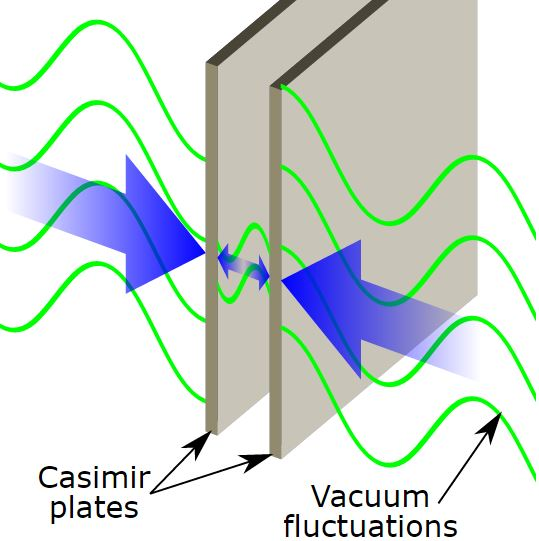
\includegraphics[width=5 cm]{pic/Casimir.jpg}
\caption{卡西米尔效应.}
\label{Casimir}
\end{center}
\end{figure}
说明. 假设两块平行金属板距离为~$d$, 且平行于~$x-y$ 平面; 它们面积相等, 为~$A$. 于是我们可得~$d$ 间隔内, 对电磁场, 单位面积上的基态能量为
\begin{align}
\frac{\langle E\rangle}{A}=2\int \frac{dk_xdk_y}{(2\pi)^2}\sum_{n=1}^\infty\frac{\hbar}{2}\omega_n=2\int \frac{dk_xdk_y}{(2\pi)^2}\sum_{n=1}^\infty\frac{\hbar}{2}c\sqrt{k^2_x+k^2_y+\left(\frac{n\pi}{d}\right)^2};
\end{align}
其中对~$z$ 方向我们采用量子力学计算结果, 对~$x, y$ 方向我们采用了周期边界条件, 即~$k=\frac{2\pi}{L}$. 上述积分值是发散的; 我们采用~zeta 正规化, 并转移到极坐标之中, 就有
\begin{align}
\frac{\langle E(s)\rangle}{A}=&\hbar\int \frac{dk_xdk_y}{(2\pi)^2}\sum_{n=1}^\infty\omega_n|\omega_n|^{-s}=\frac{\hbar c^{1-s}}{4\pi^2}\sum_n\int_0^\infty 2\pi q dq\Big|q^2+\frac{n^2\pi^2}{d^2}\Big|^{(1-s)/2}\nonumber\\
=&-\frac{\hbar^{1-s}\pi^{2-s}}{2a^{3-s}}\frac{1}{3-s}\sum_n|n|^{3-s}.
\end{align}
如此我们便可算出
\begin{align}
\frac{\langle E\rangle}{A}=\lim_{s\rightarrow0}\frac{\langle E(s)\rangle}{A}=-\frac{\hbar c\pi^2}{6a^3}\zeta(-3)=-\frac{\hbar c\pi^2}{720a^3};
\end{align}
其中用到了~$\zeta(-3)=\frac{1}{120}$. 于是卡西米尔力就是
\begin{align}
\frac{F_c}{A}=-\frac{\partial}{\partial d}\frac{\langle E\rangle}{A}=-\frac{\hbar c\pi^2}{240a^4}.
\end{align}



\subsection{单粒子态及其正交归一化分析, 坐标空间场算符对易关系, 协变对易式}


从量子力学中我们已熟知, 前文动量空间场算符的对易关系, 意味着~$a^\dag_{\bm{p}}$ 是粒子的产生算符, 即~$a^\dag_{\bm{p}}|0\rangle=|\bm{p}\rangle$. 于是可知~$\langle0|[a_{\bm{p}},a^\dag_{\bm{p}'}]|0\rangle=\langle0|a_{\bm{p}}a^\dag_{\bm{p}'}|0\rangle=\langle\bm{p}|\bm{p}'\rangle=(2\pi)^3\delta^3(\bm{p}-\bm{p}')$. 进一步地,
\begin{align}
\phi(x)|0\rangle=\phi^\dag(x)|0\rangle=\int\frac{d^3\bm{p}}{(2\pi)^3\sqrt{2E_{\bm{p}}}}e^{ipx}a^\dag_{\bm{p}}|0\rangle
=\int\frac{d^3\bm{p}}{(2\pi)^3\sqrt{2E_{\bm{p}}}}e^{ipx}|\bm{p}\rangle:=|x\rangle
\end{align}
就表示在~$x$ 点处产生一个可分解为诸动量模叠加的粒子; 注意上述量子态是洛伦兹标量, 即对任何惯性系, 都给出同样的物理. 由此可以得到\footnote{作为对比, $\delta^3(\bm{r}-\bm{r}')=\frac{1}{(2\pi\hbar)^3}\int d^3\bm{p}e^{i\bm{p}\cdot(\bm{r}-\bm{r}')/\hbar}$.}
\begin{align}
\langle x|y\rangle:=\langle0|\phi(x)\phi(y)|0\rangle=\int\frac{d^3\bm{p}}{(2\pi)^32E_{\bm{p}}}e^{-ip(x-y)}:=D(x-y)
\end{align}
即描述粒子从~$y$ 到~$x$ 的传播. 注意此传播关系亦是洛伦兹标量.

数学上我们知道, $\delta(f(x)-f(x_0))=\frac{1}{|f'(x_0)|}\delta(x-x_0)$, 故可计算得
\begin{align}
&\delta^3(\bm{p}-\bm{p}')=\delta^3(\bm{p}_b-\bm{p}'_b)\frac{dp^i_b}{dp^i}=\delta^3(\bm{p}_b-\bm{p}'_b)\gamma(1+\beta\frac{dE_{\bm{p}}}{dp^i})\nonumber\\
=&\delta^3(\bm{p}_b-\bm{p}'_b)\frac{\gamma}{E_{\bm{p}}}(E_{\bm{p}}+\beta p^i)=\delta^3(\bm{p}_b-\bm{p}'_b)\frac{E_{\bm{p}_b}}{E_{\bm{p}}};
\end{align}
其中用到了能量动量四维矢量的洛伦兹变换式~(\ref{titi}). 由上述过程可见, $E_{\bm{p}}\delta^3(\bm{p}-\bm{p}')$ 是洛伦兹不变的. 把因子平分到产生湮灭算符上, 就得~$\sqrt{2E_{\bm{p}}}a_{\bm{p}}$ 是洛伦兹标量. 在表明~K-G 场方程解~(\ref{so of kg}) 是洛伦兹标量时, 前文曾提到过这个问题, 现在得以解决.\footnote{用与第一章中描述场在实空间转动下的变化行为的语言相似的方式叙述, 就是~$U(\Lambda_p)\sqrt{2E_{\bm{p}}}a_{\bm{p}}=\sqrt{2E_{\Lambda^{-1}_p\bm{p}}}a_{\Lambda^{-1}_p\bm{p}}=\sqrt{2E_{\bm{p}}}a_{\bm{p}}$.}%; 于是有~$U(\Lambda_p)a_{\bm{p}}=\frac{\sqrt{2E_{\Lambda^{-1}_p\bm{p}}}}{\sqrt{2E_{\bm{p}}}}a_{\Lambda^{-1}_p\bm{p}}$.}
%
%\footnote{用与第一章中描述场在实空间转动下的变化行为的语言相似的方式叙述, 就是~$\sqrt{2E_{\bm{p}}}a_{\bm{p}}\rightarrow\sqrt{2E'_{\bm{p}}}a'_{\bm{p}}=\sqrt{2E_{\bm{p}}}a_{\bm{p}}= U(\Lambda_p)\sqrt{2E_{\bm{p}}}a_{\bm{p}}=\sqrt{2E_{\Lambda^{-1}_p\bm{p}}}a_{\Lambda^{-1}_p\bm{p}}$~(标量表示~$M=I$, 对比于~$\phi'(x)=U(\Lambda)\phi(x)=\phi(\Lambda^{-1}x)$); 于是有~$a'_{\bm{p}}=a_{\bm{p}}=\frac{\sqrt{2E_{\Lambda^{-1}_p\bm{p}}}}{\sqrt{2E'_{\bm{p}}}}a_{\Lambda^{-1}_p\bm{p}}=\frac{\sqrt{2E_{\Lambda^{-1}_p\bm{p}}}}{\sqrt{2E_{\bm{p}}}}a_{\Lambda^{-1}_p\bm{p}}$, 从而~$a_{\bm{p}}\rightarrow a'_{\bm{p}}=a_{\bm{p}}=U(\Lambda_p)a_{\bm{p}}=\frac{\sqrt{2E_{\Lambda^{-1}_p\bm{p}}}}{\sqrt{2E'_{\bm{p}}}}a_{\Lambda^{-1}_p\bm{p}}=\frac{\sqrt{2E_{\Lambda^{-1}_p\bm{p}}}}{\sqrt{2E_{\bm{p}}}}a_{\Lambda^{-1}_p\bm{p}}$. 注意后一表达并不构成什么表示, 而只表示一种变化关系; 如同长度等在~boost 下的行为那样; 但仍不妨与~$A'^\mu(x)=U(\Lambda)A^\mu(x)={\Lambda^\mu}_\nu A^\nu(\Lambda^{-1}x)$ 作一比较体会.}
%
%带撇读作新函数在某点, 不带读做老函数在某点
%$\sqrt{2E_{\bm{p}}}a_{\bm{p}}\rightarrow U(\Lambda_p)\sqrt{2E_{\bm{p}}}a_{\bm{p}}=\sqrt{2E_{\Lambda_p\bm{p}}}a_{\Lambda_p\bm{p}}=\sqrt{2E_{\bm{p}}}a_{\bm{p}}$, 从而~$a_{\bm{p}}=\frac{\sqrt{2E_{\Lambda_p\bm{p}}}}{\sqrt{2E_{\bm{p}}}}a_{\Lambda_p\bm{p}}$, $a_{\bm{p}}\rightarrow a_{\Lambda_p\bm{p}}=U(\Lambda_p)a_{\bm{p}}=\frac{\sqrt{2E_{\bm{p}}}}{\sqrt{2E_{\Lambda_p\bm{p}}}}a_{\bm{p}}$
%
%结结是标量, 区别于标量函数.
%
%世界上为什么会有标量, 矢量等? 因为群有平庸表示, 基本表示.
%
于是, 如下量子态~$|p^\mu\rangle:=\sqrt{2E_{\bm{p}}}a^\dag_{\bm{p}}|0\rangle=\sqrt{2E_{\bm{p}}}|\bm{p}\rangle$ 就是洛伦兹不变的; 还可得其归一化为~$\langle p|p'\rangle=2E_{\bm{p}}(2\pi)^3\delta^3(\bm{p}-\bm{p}')$. 本节中, 有了前文的知识, 就可计算出~$\langle p|x\rangle=e^{ipx},~\langle x|p\rangle=e^{-ipx}$; 还可计算出
\begin{gather}
I=\int\frac{d^3\bm{p}}{(2\pi)^32E_{\bm{p}}}|p\rangle\langle p|,~I=2E_{\bm{p}}\int d^3\bm{x}|x\rangle\langle x|.
\end{gather}
若再选定~$\langle \bm{p}|\bm{x}\rangle=e^{-i\bm{p}\cdot\bm{x}},~\langle \bm{x}|\bm{p}\rangle=e^{i\bm{p}\cdot\bm{x}}$, 以及~$\langle\bm{x}|\bm{y}\rangle=\delta^3(\bm{x}-\bm{y})$, 则还可计算出
\begin{gather}
I=\int\frac{d^3\bm{p}}{(2\pi)^3}|\bm{p}\rangle\langle\bm{p}|,~I=\int d^3\bm{x}|\bm{x}\rangle\langle\bm{x}|.
\end{gather}
类似刚才给出的~$|p\rangle$ 与~$|\bm{p}\rangle$ 的关系, 我们也可给出~$\sqrt{2E_{\bm{p}}}|x\rangle\leftrightarrow|\bm{x}\rangle$.


应用前一节我们给出的动量空间场算符的对易关系, 不难计算出坐标空间:
\begin{align}
[\phi(x),\phi(y)]&=\int\frac{d^3\bm{p}}{(2\pi)^32E_{\bm{p}}}\left[e^{-ip(x-y)}-e^{-ip(y-x)}\right]\nonumber\\
&=D(x-y)-D(y-x),\\
[\pi(x),\pi(y)]&=\int\frac{d^3\bm{p}}{(2\pi)^3}\frac{E_{\bm{p}}}{2}\left[e^{-ip(x-y)}-e^{-ip(y-x)}\right],\\
[\phi(x),\pi(y)]&=\frac{i}{2}\int\frac{d^3\bm{p}}{(2\pi)^3}\left[e^{-ip(x-y)}+e^{-ip(y-x)}\right];
\end{align}
上述第一个对易关系, 或称为协变对易关系, 是洛伦兹标量; 后两个则不是. 再应用本节给出的四维到三维的退变手续, 我们即可由上述式子读出等时对易关系
\begin{align}
[\phi(\bm{x}),\phi(\bm{y})]=0,~[\pi(\bm{x}),\pi(\bm{y})]=0,~[\phi(\bm{x}),\pi(\bm{y})]=i\delta^3(\bm{x}-\bm{y}).
\end{align}

最后, 不难解出
\begin{align}
a_{\bm{p}}&=(2\pi)^3\int d^3\bm{x}\varphi^*_{\bm{p}}(x)i\overset{\leftrightarrow}{\partial}_0\phi(x)\nonumber\\
&=\sqrt{2E_{\bm{p}}}\int d^3\bm{x}e^{ipx}\frac{1}{2}\left[\phi(x)+\frac{i\pi(x)}{E_{\bm{p}}}\right],\\
a^\dag_{\bm{p}}&=(2\pi)^3\int d^3\bm{x}\phi(x)i\overset{\leftrightarrow}{\partial}_0\varphi_{\bm{p}}(x)\nonumber\\
&=\sqrt{2E_{\bm{p}}}\int d^3\bm{x}e^{-ipx}\frac{1}{2}\left[\phi(x)-\frac{i\pi(x)}{E_{\bm{p}}}\right];
\end{align}
若先设出坐标空间场量的含时对易关系, 从上式亦是可以推出动量空间的对易式的.


\subsection{狭义相对论微观因果律对量子场论的要求: 粒子自旋与对易性/对称性/统计的关系}


狭义相对论表明, 类时或类光间隔的两个事件, 可以建立信号联接; 而类空间隔的事件是不可以的, 后者将失去确定的先后次序. 这称为狭义相对论所界定的微观世界的因果律. 反映在量子场论上, 这就是要求, 类空间隔两点上的力学量算符, 必须是互相对易的, 即
\begin{align}
[\mathcal{O}(x),\mathcal{O}(y)]=0,~\textrm{when}~(x-y)^2<0.
\end{align}
容易看出, 此条件反映在组成力学量算符的场算符上, 就是要求,
\begin{center}
场算符所取的对易关系类型, 要使得在类空间隔内, 场的采取同样对易关系的协变运算式结果为零.
\end{center}

由上一小节的计算我们已知~$[\phi(x),\phi(y)]=D(x-y)-D(y-x)$; 在类空间隔内, 此对易式的值的确是等于零的. 同时也可看出, 若将场量取为反对易式, 则类空间隔内它们的反对易结果显然不为零. 是故自旋为零的标量场必取对易关系. 同样, 在下一章狄拉克场中我们也将看到, 对具有~$1/2$ 自旋的粒子, 在类空间隔内, 其采取反对易式的场的协变运算式结果为零. 是故自旋为~$1/2$ 的粒子必取反对易关系.

进一步, 我们将发现, 因狭义相对论因果律的要求, 具有整数自旋的粒子, 必须被赋予对易关系; 粒子波函数对粒子交换是对称的, 粒子系满足玻色-爱因斯坦统计; 这样的粒子称为玻色子. 而具有半奇数自旋的粒子, 必须被赋予反对易关系; 粒子波函数对粒子交换是反对称的, 粒子系满足费米-狄拉克统计; 这样的粒子称为费米子.




\subsection{费曼传播子}

前面我们已知道~$\langle x|y\rangle=D(x-y)$ 表示粒子从~$y$ 到~$x$ 的传播; 但其中我们并没有计及时间的先后. 考虑进时间先后的传播子~$D_F(x-y):=\langle0|T\phi(x)\phi(y)|0\rangle$, 称为费曼传播子. 另外, $D_R(x-y):=\theta(x^0-y^0)\langle0|[\phi(x),\phi(y)]|0\rangle$ 称为推迟格林函数. 下面, 我们以费曼传播子为例, 来对其进行计算.
\begin{align}
&D_F(x-y)=\langle0|T\phi(x)\phi(y)|0\rangle\nonumber\\
=&\theta(x^0-y^0)\langle0|\phi(x)\phi(y)|0\rangle+\theta(y^0-x^0)\langle0|\phi(y)\phi(x)|0\rangle\nonumber\\
=&\theta(x^0-y^0)\int\frac{d^3\bm{p}}{(2\pi)^32E_{\bm{p}}}e^{-ip(x-y)}+\theta(y^0-x^0)\int\frac{d^3\bm{p}}{(2\pi)^32E_{\bm{p}}}e^{-ip(y-x)}\nonumber\\
=&\theta(x^0-y^0)\int\frac{d^3\bm{p}}{(2\pi)^32E_{\bm{p}}}e^{-ip(x-y)}\Big|_{p^0=E_{\bm{p}}}\nonumber\\
&-\theta(y^0-x^0)\int\frac{d^3\bm{p}}{(2\pi)^3(-2E_{\bm{p}})}e^{-ip(x-y)}\Big|_{p^0=-E_{\bm{p}}}\nonumber
%=&\int\frac{d^3\bm{p}}{(2\pi)^3}\int\frac{dp^0}{2\pi i}\frac{-1}{p^2-m^2}e^{-i(x-y)}~\textrm{with~Feynman~prescription}\nonumber\\
%=&\int\frac{d^4p}{(2\pi)^4}\frac{i}{p^2-m^2}e^{-i(x-y)}~\textrm{with~Feynman~prescription};
\end{align}
\begin{align}
%&D_F(x-y)=\langle0|T\phi(x)\phi(y)|0\rangle\nonumber\\
%=&\theta(x^0-y^0)\langle0|\phi(x)\phi(y)|0\rangle+\theta(y^0-x^0)\langle0|\phi(y)\phi(x)|0\rangle\nonumber\\
%=&\theta(x^0-y^0)\int\frac{d^3\bm{p}}{(2\pi)^32E_{\bm{p}}}e^{-ip(x-y)}+\theta(y^0-x^0)\int\frac{d^3\bm{p}}{(2\pi)^32E_{\bm{p}}}e^{-ip(y-x)}\nonumber\\
%=&\theta(x^0-y^0)\int\frac{d^3\bm{p}}{(2\pi)^32E_{\bm{p}}}e^{-ip(x-y)}\Big|_{p^0=E_{\bm{p}}}\nonumber\\
%&-\theta(y^0-x^0)\int\frac{d^3\bm{p}}{(2\pi)^3(-2E_{\bm{p}})}e^{-ip(x-y)}\Big|_{p^0=-E_{\bm{p}}}\nonumber\\
=&\int\frac{d^3\bm{p}}{(2\pi)^3}\int\frac{dp^0}{2\pi i}\frac{-1}{p^2-m^2}e^{-i(x-y)}~\textrm{with~Feynman~prescription}\nonumber\\
=&\int\frac{d^4p}{(2\pi)^4}\frac{i}{p^2-m^2}e^{-i(x-y)}~\textrm{with~Feynman~prescription};
\end{align}
其中用到了留数定理~$\oint_l f(z)dz=2\pi i\sum_k f(a_k)$, 而积分围道的选择表示在图~\ref{feynman} 中, 称为费曼惯例.
\begin{figure}[!h]
\begin{center}
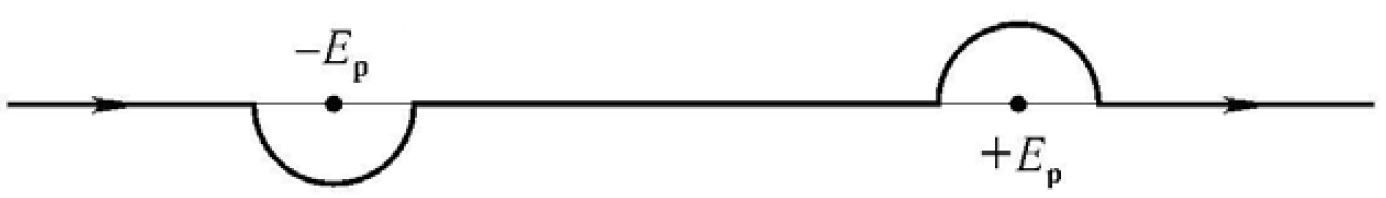
\includegraphics[width=7 cm]{pic/feynman.jpg}
\caption{费曼惯例: 费曼传播子积围道的选取.}
\label{feynman}
\end{center}
\end{figure}

显然, 对~$\int\frac{d^4p}{(2\pi)^4}\frac{i}{p^2-m^2}e^{-i(x-y)}$ 的积分围道的不同选择, 将给出不同的传播子. 若我们将其积分围道选取为图~\ref{ret}, 则就得出推迟格林函数.
\begin{figure}[!h]
\begin{center}
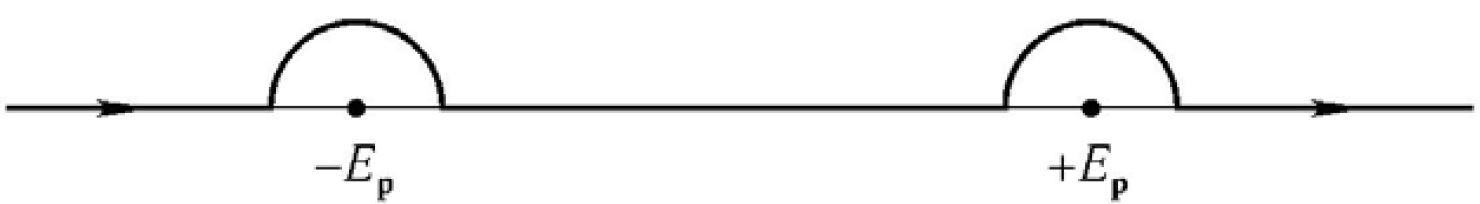
\includegraphics[width=7 cm]{pic/ret.jpg}
\caption{推迟势积分围道的选取.}
\label{ret}
\end{center}
\end{figure}

\noindent 对于费曼传播子, 一般我们又会采用如下记法:
\begin{align}
D_F(x-y)=\int\frac{d^4p}{(2\pi)^4}\frac{i}{p^2-m^2+i\epsilon}e^{-ip(x-y)},
\end{align}
或称为~$\epsilon$ 惯例.

对于日后相互作用场中的计算来讲, 费曼传播子, 基本上是自由场论中最重要的结果.

%传播子是否涉及到虚过程?



\subsection{复标量场: 零自旋有质量有荷, $\pi^\pm$ 介子}

我们已知, 本章以前部分讲述的实标量场, 描述的是~$\pi^0$ 介子. 还有一类带正负电荷的介子, 记为~$\pi^\pm$; 由前章内容知, 描述它们的即为复标量场. 复标量场的拉氏密度, 以及由之导致的场的运动方程, 进而场的解为:
\begin{gather}
\mathcal{L}=\partial_\mu\phi^\dag\partial^\mu\phi-m^2\phi^\dag\phi,\\
(\partial^2+m^2)\phi=0,~(\partial^2+m^2)\phi^\dag=0;\\
\phi(x)=\int\frac{d^3\bm{p}}{(2\pi)^3\sqrt{2E_{\bm{p}}}}\left(a_{\bm{p}}e^{-ipx}+b^\dag_{\bm{p}}e^{ipx}\right),\\
\phi^\dag(x)=\int\frac{d^3\bm{p}}{(2\pi)^3\sqrt{2E_{\bm{p}}}}\left(a^\dag_{\bm{p}}e^{ipx}+b_{\bm{p}}e^{-ipx}\right);
\end{gather}
其中~$a^\dag_{\bm{p}}$ 与~$b^\dag_{\bm{p}}$ 即描述带分别带正负电荷的两种粒子. 本场的正则动量以及哈氏密度就是
\begin{gather}
\pi=\frac{\partial\mathcal{L}}{\partial\dot{\phi}}=\dot{\phi}^\dag,~\pi^\dag=\frac{\partial\mathcal{L}}{\partial\dot{\phi}^\dag}=\dot{\phi};\\
\mathcal{H}=\pi\dot{\phi}+\pi^\dag\dot{\phi}^\dag-\mathcal{L}.
\end{gather}
赋予本场如下对易关系, 即可实现体系的量子化:
\begin{gather}
[a_{\bm{p}},a^\dag_{\bm{p}'}]=(2\pi)^3\delta^3(\bm{p}-\bm{p}'),~[b_{\bm{p}},b^\dag_{\bm{p}'}]=(2\pi)^3\delta^3(\bm{p}-\bm{p}');\\
\Leftrightarrow~[\phi(\bm{x}),\pi(\bm{y})]=i\delta^3(\bm{x}-\bm{y}),~[\phi^\dag(\bm{x}),\pi^\dag(\bm{y})]=i\delta^3(\bm{x}-\bm{y});
\end{gather}
其它的对易皆为零. 场的协变对易关系很容易读出为~
\begin{gather}
[\phi(x),\phi(y)]=0,~[\phi^\dag(x),\phi^\dag(y)]=0,\\
[\phi(x),\phi^\dag(y)]=D_a(x-y)-D_b(y-x).
\end{gather}
复标量场的大部分力学性质与实标量场的是对应一致的; 我们主要研究复标量场所带的规范荷. 复标量场对应于整体规范不变的守恒流密度为
\begin{align}
j^\mu_{(q)}=&\frac{q}{i}\left(\frac{\partial\mathcal{L}}{\partial\partial_\mu\phi}\phi-\phi^\dag\frac{\partial\mathcal{L}}{\partial\partial_\mu\phi^\dag}\right)\nonumber\\
=&iq(\phi^\dag\partial^\mu\phi-\phi\partial_\mu\phi^\dag);
\end{align}
这是我们在分析力学中我们就已求出过的. 于是我们可以求出本场的总守恒荷为
\begin{align}
Q=&\int d^3\bm{x}j^0_{(q)}=iq\int d^3\bm{x}(\phi^\dag\partial^0\phi-\phi\partial_0\phi^\dag)\nonumber\\
=&q\int\frac{d^3\bm{p}}{(2\pi)^3}(a^\dag_{\bm{p}}a_{\bm{p}}-b^\dag_{\bm{p}}b_{\bm{p}})
\end{align}
由此确认, $a^\dag_{\bm{p}}$ 与~$b^\dag_{\bm{p}}$ 描述的粒子荷性的确相反.












